\chapter{Energy web}

%%%%%%%%%%%%
% Content
%%%%%%%%%%%%
\section{Cos'è Energy Web}
\gls{ew} è un progetto nato nel 2017 con sede in Zugo, Svizzera \cite{wiki:ew-history}. 
Ad affiancarlo e dargli valore vi sono molti partner commerciali, comprese aziende molto conosciute nel settore energetico \cite{wiki:ew-affiliate}. \\
L'obiettivo prefissato da \gls{ew} è quello di spingere per uno sviluppo del settore che punti verso un abbassamento delle emissioni di carbonio e che sia in grado di gestire la decentralizzazione del mercato delle risorse.
Per farlo, \gls{ew} utilizza tecnologie distribuite e open-source dalle quali partire per realizzare un'infrastruttura commerciale specifica per l'ambito energetico \cite{wiki:ew-about}. \\
Nel 2019, \gls{ew} ha rilasciato \gls{ewc}, una blockchain pubblica basata su Ethereum, sulla quale si basa l'intero ecosistema di \gls{ew}: \gls{ewdos}.

\section{EW-DOS}
Il cuore del progetto di \gls{ew} è \gls{ewdos}, un'infrastruttura digitale open-source ad accesso pubblico e decentralizzato. \\
L'idea è quella di fornire un insieme di strumenti e servizi che rendano il più semplice possibile lo sviluppo di \gls{dapp} mirate al settore energetico, 
anche se, ovviamente, le varie tecnologie possono essere applicate anche ad ambiti più generici. \\
L'intero sistema è stato pensato come tre strati sovrapposti, in cui ogni strato si basa su quello sottostante per implementare ulteriori funzionalità, come mostrato in \autoref{lab:ew-dos}. \\

I tre strati sono:
\begin{itemize}
    \item Trust - \gls{ewc}
    \item Utility - Servizi e astrazioni sopra la blockchain
    \item Toolkit - Frameworks e toolkit per la costruzione di applicazioni
\end{itemize}

\begin{figure}[h]
    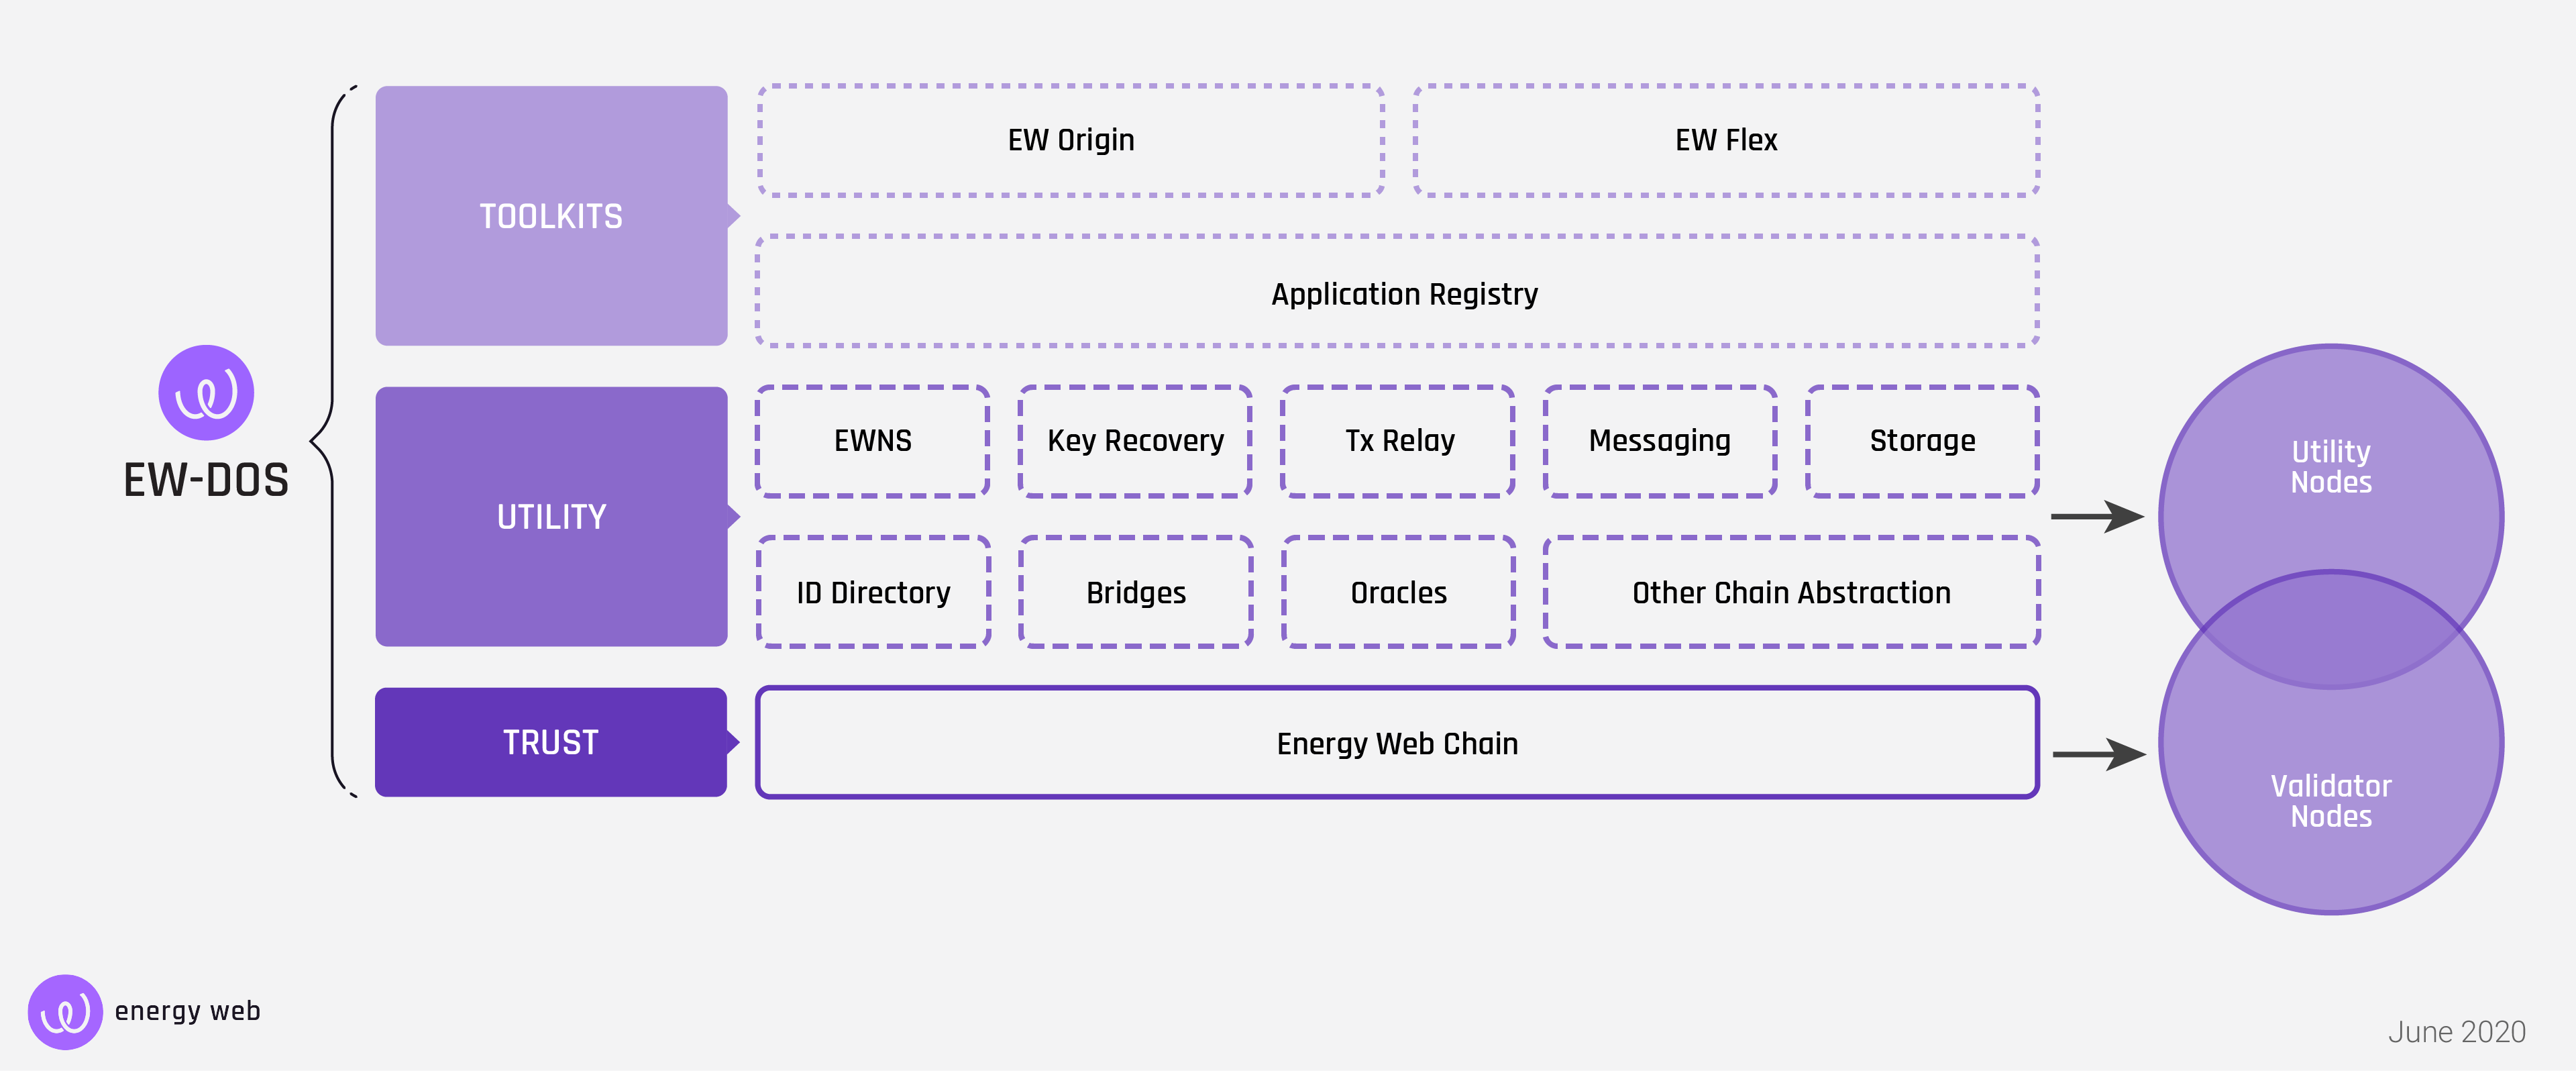
\includegraphics[width=13cm]{ew-dos}
    \centering
    \caption{Visualizzazione della struttura di \gls{ewdos} \cite{img:ew-dos}}
    \label{lab:ew-dos}
\end{figure}

\section{Trust}
Il livello Trust comprende la \gls{ewc} (cfr. \autoref{cap:ew}), 
il cui ruolo principale è quello di assicurare che ci sia consenso sui dati e che tutte le applicazioni e gli smart contracts si comportino in maniera deterministica. \\
Si tratta di una blockchain basata su Ethereum, \gls{evm} inclusa, e rispetta tutti gli \gls{erc}. \\
Il token digitale per il pagamento delle transazioni e dei servizi offerti dalla piattaforma è l'\gls{ewt} e l'algoritmo di consenso è il \gls{poa}. \\
È presente anche una test-net, chiamata Volta, usata per testare i progetti e le applicazioni prima di lanciarle sulla main-net. 

\section{Utility}
Il livello di utility è composto da un insieme di servizi basati sulla \gls{ewc} che hanno lo scopo di rendere quanto più accessibile e invitante possibile l'intera infrastruttura per gli sviluppatori di DApp,
ed inoltre mettendo a disposizione un gran numero di smart contracts per il backend e di librerie per il frontend \cite{art:ew-dos}. \\
Come anticipato, il pagamento di servizi del livello di Utility della piattaforma vengono pagati in EWT. \\
I nodi della blockchain che forniscono queste funzionalità sono chiamati Utility Nodes, e vengono ricompensati attraverso il meccanismo dello Staking (cfr. \autoref{sec:staking}).\\

È possibile individuare tre ampie categorie di servizi:
\begin{itemize}
    \item Esperienza dell'utente finale
    \item Interoperabilità Multipiattaforma
    \item Performance delle applicazioni
\end{itemize}

\subsection{Esperienza dell'utente finale}
\begin{itemize}
    \item \gls{ewns} - Similmente ad un DNS, associa domini arbitrari ad indirizzi sulla blockchain
    \item DID Key Recovery - Permette il recupero della propria DID  (cfr. \autoref{sec:did})
    nel caso si fosse persa la chiave privata
    \item Transaction Relay - Servizio che fa da intermediario fra un cliente e la blockchain, nascondendo l'utilizzo della stessa e simulando una più tradizionale interazione client-server
\end{itemize}

\subsection{Interoperabilità Multipiattaforma}
\begin{itemize}
    \item Bridges - Consente il trasferimento di token fra blockchain diverse. Attualmente è utilizzato per collegare \gls{ewc} con Ethereum
    \item Oracles - Particolari nodi che è possibile consultare con il protocollo Chainlink per ricevere dati di eventi esterni alla blockchain \cite{art:oracles} \cite{wiki:oracles} 
\end{itemize}

\subsection{Performance delle applicazioni}
\begin{itemize}
    \item Identity Directory - Smart contract che contiene tutti le \gls{did}
    \item Messaging - Un sistema di messaggistica che sfrutta le \gls{did} per assicurare validità ed autenticità dei messaggi
    \item Storage - L'utilizzo di sistemi di storage distribuiti esterni, come IPFS \cite{wiki:ipfs}  rende possibile limitare al minimo indispensabile la quantità di dati salvati sulla blockchain
\end{itemize}

\section{Toolkit}
Il livello toolkit comprende una serie di framework ed applicazioni di esempio utili per realizzare \gls{dapp} che sfruttino al massimo le funzionalità di \gls{ewdos} \cite{art:ew-dos}.
Sebbene siano pensati per il settore energetico, la loro natura open-source li rende ottime basi di partenza per costruire soluzioni anche per altri ambiti.

\subsection{Application Registry}
Architettura in grado creare registri di \gls{did} che verifichino che soddisfino la condizione specificata, come ad esempio la località geografica o il possesso di una certa qualifica.

Questo registro sarà poi utilizzato da una \gls{dapp} per creare un servizio di autorizzazione e autenticazione. 

Ogni \gls{dapp} deve fare riferimento ad un Application Registry, che può essere riutilizzato in più applicazioni.

\subsection{EW origin}
Framework per sviluppare applicazioni che supportino il tracciamento, la trasmissione e il conferimento di \gls{eac} alle \gls{res} secondo gli standard del settore. 

I due attori principali sono il Registry e l'Issuer. 
Il primo salva e amministra le informazioni legate ad utenti e \gls{der}, con la possibilità di mantenere dati potenzialmente sensibili off-chain, cioè utilizzando dello storage al di fuori della blockchain.
Il secondo potrà essere utilizzato dalle autorità competenti per coniare nuovi \gls{eac} che siano tracciabili, con una implementazione basata sullo standard ERC-1155.

\subsection{EW flex}
Software open source attualmente in sviluppo per la gestione dei \gls{der} e le operazioni che li coinvolgono, 
permettendone una facile connessione alla rete e sottoponendo le offerte ad un operatore autorizzato \cite{art:ew-dos}. \\

Sarà composto dai seguenti moduli:

\begin{itemize}
    \item Flex Nodes - Cluster di nodi che eseguono materialmente la business logic che gestisce offerta e domanda, e le accoppia secondo quanto stabilito dall'operatore responsabile.
    \item Flex Clients - Insieme di tutti i \gls{der} che partecipano al mercato dell'energia, inclusi dispositivi \gls{iot}
    \item Flex Bridge - Modulo che permette la comunicazione e la coordinazione con gli operatori della rete elettrica
    \item Flex Governance - Serie di smart contracts che governano i Flex Nodes. Permettono agli enti predisposti di imporre le regolamentazioni vigenti
\end{itemize}